\subsection{Hồi quy tuyến tính}
\paragraph{}{Các kiến thức trong phần này được trích dẫn từ sách Mathematics for Machine Learning \cite{deisenroth2020mathematics} - Đại học Cambridge và một số blog khác.} 
\label{label:lr}
\subsubsection{Hồi quy tuyến tính (Linear regression)}
\paragraph{}{\textbf{Mô hình toán học}}

Hồi quy tuyến tính \cite{mlcoban-linear-regression} là một phương pháp thống kê dùng để dự báo mối quan hệ giữa biến độc lập (biến đầu vào \( x_i \)) và biến phụ thuộc (biến đầu ra \( y \)). Mô hình tuyến tính tổng quát có dạng:

\begin{equation}
y = w_0 + w_1x_1 + w_2x_2 + \dots + w_nx_n + \varepsilon
\end{equation}

Trong đó:
\begin{itemize}
    \item \( y \) là biến phụ thuộc (đầu ra cần dự đoán),
    \item \( x_1, x_2, \dots, x_n \) là các biến độc lập (đặc trưng đầu vào),
    \item \( w_0, w_1, \dots, w_n \) là các hệ số hồi quy (cần tìm),
    \item \( \varepsilon \) là nhiễu ngẫu nhiên.
\end{itemize}

\paragraph{}{\textbf{Hàm mất mát}}

Để đo lường sai số giữa giá trị thực tế và giá trị dự đoán, ta sử dụng hàm mất mát bình phương trung bình (Mean Squared Error - MSE):

\begin{equation}
J(w) = \frac{1}{m} \sum_{i=1}^{m} (y_i - \hat{y}_i)^2
\end{equation}

với:
\begin{itemize}
    \item \( m \) là số lượng mẫu dữ liệu,
    \item \( y_i \) là giá trị thực tế của mẫu thứ \( i \),
    \item \( \hat{y}_i \) là giá trị dự đoán của mẫu thứ \( i \), được tính theo công thức:
\end{itemize}

\begin{equation}
\hat{y}_i = w_0 + w_1x_{i1} + w_2x_{i2} + \dots + w_nx_{in}
\end{equation}

Mục tiêu của mô hình là tìm các tham số \( w \) sao cho hàm mất mát \( J(w) \) đạt giá trị nhỏ nhất. Có hai cách tiếp cận chính:

\begin{enumerate}
    \item \textbf{Phương pháp đạo hàm và giải hệ phương trình}  

    Khi số lượng biến không quá lớn, ta có thể tìm nghiệm bằng cách giải phương trình đạo hàm bằng không:

    \begin{equation}
    w = (X^TX)^{-1}X^Ty
    \end{equation}

    với \( X \) là ma trận đặc trưng của dữ liệu đầu vào.

    \item \textbf{Gradient Descent (Hạ Gradient)}

    Khi số lượng biến lớn, ta có thể sử dụng phương pháp hạ gradient để tối ưu:

    \begin{itemize}
        \item \textbf{Gradient của hàm mất mát theo \( w_j \):}
        \begin{equation}
        \frac{\partial J}{\partial w_j} = -\frac{2}{m} \sum_{i=1}^{m} (y_i - \hat{y}_i) x_{ij}
        \end{equation}
        
        \item \textbf{Cập nhật tham số \( w_j \) theo thuật toán Gradient Descent:}
        \begin{equation}
        w_j := w_j - \alpha \frac{\partial J}{\partial w_j}
        \end{equation}
    \end{itemize}

    trong đó:
    \begin{itemize}
        \item \( \alpha \) là tốc độ học (learning rate),
        \item quá trình này lặp lại cho đến khi hội tụ.
    \end{itemize}

\end{enumerate}
\subsubsection{Lý thuyết tìm cực trị có điều kiện Lagrange}

\paragraph{}{Giả sử ta cần tìm cực trị của hàm số \( f(x_1, x_2, ..., x_n) \) với ràng buộc:}
\[
g(x_1, x_2, ..., x_n) = 0
\]
\paragraph{}{Phương pháp nhân tử Lagrange xây dựng hàm:}
\[
\mathcal{L}(x_1, x_2, ..., x_n, \lambda) = f(x_1, x_2, ..., x_n) + \lambda g(x_1, x_2, ..., x_n)
\]
trong đó \( \lambda \) là nhân tử Lagrange.

\paragraph{}{Điều kiện cần để tìm cực trị là:}
\[
\nabla \mathcal{L} = 0 \Rightarrow  
\begin{cases}  
\frac{\partial \mathcal{L}}{\partial x_1} = 0 \\  
\frac{\partial \mathcal{L}}{\partial x_2} = 0 \\  
\vdots \\  
\frac{\partial \mathcal{L}}{\partial x_n} = 0 \\  
\frac{\partial \mathcal{L}}{\partial \lambda} = g(x_1, x_2, ..., x_n) = 0  
\end{cases}
\]
\paragraph{}{Giải hệ phương trình trên giúp tìm nghiệm tối ưu của bài toán có ràng buộc.}

\subsubsection{Hồi quy Ridge}
\label{label:ridge-math}
\paragraph{}{Hồi quy Ridge \cite{phamkhanh-ridge-regression} là bài toán tối ưu có ràng buộc:}
\[
\min_{\beta} \sum_{i=1}^{n} (y_i - X_i\beta)^2 \quad \text{với điều kiện} \quad \sum_{j=1}^{p} \beta_j^2 \leq C
\]
\paragraph{}{Điều kiện ràng buộc \( \sum_{j=1}^{p} \beta_j^2 < C \) cho thấy nghiệm tối ưu sẽ bị hạn chế về độ lớn. Trong không gian đa chiều thì điều kiện ràng buộc có miền xác định là một khối cầu có tâm là gốc tọa độ và bán kính \( \sqrt{C} \). Đây chính là một cơ chế kiểm soát mà \textit{thành phần điều chuẩn} đã áp đặt lên các biến đầu vào.}
\paragraph{}{Sử dụng phương pháp Lagrange, ta xây dựng hàm:}
\[
\mathcal{L}(\beta, \lambda) = \sum_{i=1}^{n} (y_i - X_i\beta)^2 + \lambda \left( \sum_{j=1}^{p} \beta_j^2 - C \right)
\]
\paragraph{}{Lấy đạo hàm theo \( \beta \):}
\[
\frac{\partial \mathcal{L}}{\partial \beta} = -2X^T(y - X\beta) + 2\lambda \beta = 0
\]
\paragraph{}{Giải phương trình trên, ta thu được nghiệm tối ưu:}
\[
\beta_{ridge} = (X^TX + \lambda I)^{-1} X^Ty
\]
\textbf{So với hồi quy tuyến tính thông thường (OLS):}

\begin{itemize}
\item{Khi $X^TX$ gần suy biến, việc tính $\beta_{OLS} = (X^TX)^{-1} X^Ty$ không ổn định, dẫn đến ước lượng $\beta_{OLS}$ có phương sai lớn.}

\item Hồi quy Ridge thay thế $X^TX$ bằng $X^TX + \lambda I$, với $\lambda > 0$, giúp Ma trận $X^TX + \lambda I$ luôn dương xác định và Việc tính nghịch đảo trở nên ổn định hơn.Phương sai của ước lượng giảm, cho ra $\beta_{ridge}$ ổn định hơn.
\end{itemize}
\subsubsection{Hồi quy Lasso}
\label{label:lasso-math}
\paragraph{}{Lasso Regression \cite{stackexchange-lasso} là một phương pháp hồi quy tuyến tính có điều chuẩn (regularization), được sử dụng để cải thiện hiệu suất của mô hình bằng cách giảm hiện tượng quá khớp (overfitting) thông qua công thức:}

\begin{equation} \label{eq:lasso}
    \min_{\beta} \sum_{i=1}^{n} (y_i - X_i\beta)^2 \quad \text{với điều kiện} \quad \sum_{j=1}^{p} |\beta_j| \leq C
\end{equation}

\begin{itemize}
    \item $C$ là hằng số dương, liên quan đến $\lambda$. Khi $\lambda$ lớn, $t$ nhỏ và ngược lại.
    \item Ràng buộc $\sum_{j=1}^p |\beta_j| \le C$ giới hạn tổng giá trị tuyệt đối của các hệ số $\beta_{j}$, tương ứng với chuẩn L1.
\end{itemize}

Mô hình cần tối ưu hàm sai số với điều kiện là phải thỏa ràng buộc đã đặt ra. 

\begin{figure}[H]
    \centering
    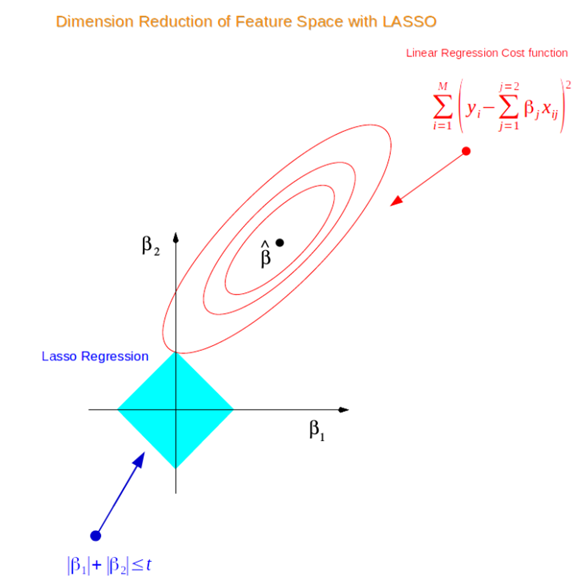
\includegraphics[width=0.7\linewidth]{img/geometry_lasso.png}
    \caption{}
    \label{fig:geometry_lasso}
\end{figure}

Lấy ví dụ với trường hợp chỉ có 2 đặc trưng, tức là chỉ có 2 hệ số $\beta_{1}, \beta_{2}$. Khi đó, không gian của $\beta$ là một mặt phẳng 2 chiều, với trục hoành là $\beta_{1}$ và trục tung là $\beta_{2}$. Ta tiến hành giảm sai số dự đoán sao cho tổng giá trị tuyệt đối của các hệ số \( \beta_j \) không được vượt quá một ngưỡng nào đó, ví dụ \( |\beta_1| + |\beta_2| \leq t \). Các giá trị của \( \beta_1 \) và \( \beta_2 \) bị giới hạn trong một khu vực có dạng hình thoi và hình thoi này có các đỉnh tại các trục

Hàm mất mát của mô hình được biểu diễn bằng các vòng tròn hoặc elip (gọi là đường đồng mức), với tâm là điểm tối ưu của hồi quy thông thường (OLS). Các elip này sẽ mở rộng từ tâm cho đến khi chạm vào biên của hình thoi (vừa đủ thỏa ràng buộc nhưng vần gần OLS nhất). Hình thoi có các góc nhọn tại các trục (nơi \( \beta_1 = 0 \) hoặc \( \beta_2 = 0 \)). Khi elip mở rộng, nó thường chạm vào các góc nhọn này trước vì các góc nhọn "nhô ra"  xa hơn so với các cạnh. Đó là vì sao đôi lúc Lasso có thể loại bỏ hoàn toàn một vài đặc trưng đóng góp cho mô hình.

\paragraph{Sử dụng phương pháp Lagrange} Ta xây dựng hàm mất mát từ (\ref{eq:lasso}):

\[
\mathcal{L}(\beta, \lambda) = \sum_{i=1}^n \left(y_i - \left(\beta_0 + \sum_{j=1}^p \beta_j x_{ij}\right)\right)^2 + \lambda \sum_{j=1}^p |\beta_j|
\]

\paragraph{Các bước cập nhật tham số trong Lasso}
Việc tối thiểu hóa hàm mất mát của Lasso không có nghiệm dạng đóng (tính nghiệm trực tiếp) như hồi quy tuyến tính thông thường, do thành phần điều chuẩn L1 (\( \lambda \|\boldsymbol{\beta}\|_1 \)) không khả vi tại \( \beta_j = 0 \). Một phương pháp phổ biến để giải bài toán này là sử dụng thuật toán \textit{Coordinate Descent}, trong đó các tham số \( \beta_0 \) và \( \boldsymbol{\beta} \) được cập nhật lần lượt từng thành phần.
\begin{enumerate}
    \item \textbf{Cập nhật hệ số chặn \( \beta_0 \)}: Coi \( \boldsymbol{\beta} \) là cố định, ta tối thiểu hóa hàm mất mát theo \( \beta_0 \). Kết quả là:
    \[
    \beta_0 = \frac{1}{n} \sum_{i=1}^n \left(y_i - \sum_{j=1}^p \beta_j x_{ij}\right)
    \]
    Dưới dạng ma trận, điều này tương đương với:
    \[
    \beta_0 = \frac{1}{n} \mathbf{1}^T (\mathbf{y} - \mathbf{X} \boldsymbol{\beta})
    \]
    Bước này đảm bảo rằng trung bình của các giá trị dự đoán khớp với trung bình của \( \mathbf{y} \).
    
    \item \textbf{Cập nhật từng hệ số \( \beta_j \)}: Coi \( \beta_0 \) và các \( \beta_k \) (với \( k \neq j \)) là cố định, ta tối thiểu hóa hàm mất mát theo \( \beta_j \). Do thành phần L1, nghiệm của \( \beta_j \) có dạng một hàm \textit{soft-thresholding}:
    \[
    \beta_j = S\left( \frac{1}{n} \sum_{i=1}^n x_{ij} r_{i(j)}, \frac{\lambda}{n} \right)
    \]
    Trong đó:
    \begin{itemize}
        \item \( r_{i(j)} = y_i - \beta_0 - \sum_{k \neq j} \beta_k x_{ik} \) là phần dư (residual) của mẫu \( i \) khi bỏ qua đóng góp của đặc trưng \( j \).
        \item \( S(z, \gamma) \) là hàm soft-thresholding, được định nghĩa như sau:
        \[
        S(z, \gamma) = 
        \begin{cases} 
        z - \gamma & \text{nếu } z > \gamma \\
        0 & \text{nếu } |z| \leq \gamma \\
        z + \gamma & \text{nếu } z < -\gamma 
        \end{cases}
        \]
    \end{itemize}
    Dưới dạng ma trận, ta có thể tính \( \mathbf{r}_{(j)} = \mathbf{y} - \beta_0 \mathbf{1} - \mathbf{X}_{-j} \boldsymbol{\beta}_{-j} \), trong đó \( \mathbf{X}_{-j} \) là ma trận \( \mathbf{X} \) bỏ cột \( j \), và \( \boldsymbol{\beta}_{-j} \) là vector \( \boldsymbol{\beta} \) bỏ thành phần \( j \). Khi đó:
    \[
    \beta_j = S\left( \frac{1}{n} \mathbf{x}_j^T \mathbf{r}_{(j)}, \frac{\lambda}{n} \right)
    \]
    với \( \mathbf{x}_j \) là cột \( j \) của ma trận \( \mathbf{X} \).
\end{enumerate}

Thuật toán Coordinate Descent đảm bảo rằng hàm mất mát giảm dần qua mỗi bước, và cuối cùng hội tụ đến nghiệm tối ưu của Lasso. Điểm đặc biệt của bước cập nhật \( \beta_j \) là hàm soft-thresholding có thể ép \( \beta_j \) về 0 nếu giá trị trung gian \( \frac{1}{n} \mathbf{x}_j^T \mathbf{r}_{(j)} \) nhỏ hơn ngưỡng \( \frac{\lambda}{n} \), điều này giải thích tại sao Lasso có khả năng lựa chọn đặc trưng.

\paragraph{So sánh Lasso Regression với hồi quy tuyến tính thông thường (OLS)}

\begin{itemize}
    \item  Lasso có khả năng tự động lựa chọn đặc trưng nhờ thành phần điều chuẩn L1. Trong khi đó, OLS không có cơ chế điều chuẩn, nên tất cả các đặc trưng đều được giữ lại, kể cả những đặc trưng không có ý nghĩa, điều này có thể làm tăng độ phức tạp của mô hình.
    
    \item Lasso giúp giảm hiện tượng quá khớp (overfitting) bằng cách giới hạn tổng giá trị tuyệt đối của các hệ số \( \beta_j \) thông qua hệ số điều chuẩn $\lambda$. Ngược lại, OLS không có điều chuẩn, nên nếu dữ liệu có nhiều đặc trưng hoặc các đặc trưng có tương quan cao, mô hình có thể học quá chi tiết trên tập huấn luyện, dẫn đến hiệu suất kém trên tập kiểm tra.
    
    \item  OLS có nghiệm dạng đóng, tức là ta có thể tính trực tiếp các hệ số \( \boldsymbol{\beta} \) bằng công thức \( \boldsymbol{\beta} = (\mathbf{X}^T \mathbf{X})^{-1} \mathbf{X}^T \mathbf{y} \). Trong khi đó, Lasso không có nghiệm dạng đóng do thành phần L1 không khả vi tại 0, nên cần sử dụng các phương pháp lặp như Coordinate Descent để tìm nghiệm, dẫn đến quá trình đạo hàm phức tạp hơn.
    
    \item  Trong các bài toán có số đặc trưng lớn (nhiều hơn số mẫu), OLS có thể gặp vấn đề vì ma trận \( \mathbf{X}^T \mathbf{X} \) không khả nghịch (do ma trận không vuông), dẫn đến không thể tính được nghiệm. Lasso, nhờ điều chuẩn L1 nó thu nhỏ các hệ số và loại bỏ các đặc trưng không cần thiết, làm giảm chiều dữ liệu hiệu quả.
\end{itemize}


